\problemWithTimeMem{黑白三消2}{1 second}{1024MB}

\textbf{埃森哲全球员工约50万名,在全球50多个国家设有分公司,为遍布120多个国家的客户提供服务。}

埃森哲曾为新加坡樟宜机场部署的 AI 导航系统,通过融合计算机视觉、实时数据分析和 AI 算法,为旅客提供精准、动态的导航服务,显著提升了机场运营效率和旅客体验。刚从智能流水线转岗到机场传感器架构师的 Capps 又遇到了新的难题:

现有 $n$ 个白色传感器和 $m$ 个黑色传感器将放置到机场里,机场可以简化成一个二维网格,需要同时满足:

- 任何两个传感器不能放到同一个点。

- 任何两个传感器的连线上不能有其他传感器。

- 这 $n$ + $m$ 个传感器在网格上的凸包顶点由 $n$ 个白色传感器和 $0$ 个黑色传感器组成。

\textbf{凸包}:指在平面上包含所有给定点集的最小凸多边形。

\mysec{Input}

一行两个正整数 $n$ $(3\leqslant n \leqslant 500)$, $m$ $(0 \leqslant m \leqslant 500)$。

\mysec{Output}

输出 $n+m$ 行,每行两个整数 $x_i$, $y_i$ $(0 \leqslant x_i, y_i \leqslant 10^9)$ 描述第 $i$ 个传感器的坐标,并且点集的凸包上恰好有 $n$ 个点,不需要关心点的输出顺序,\textbf{如果有多种方案均符合题意,输出任意一种均为正确}。

\ACMIO{Sample 1}{%
3 4
}
{%
3 0

3 1

4 2

2 3

1 4

2 4

6 5
}

\mysec{Hint}

样例的图:

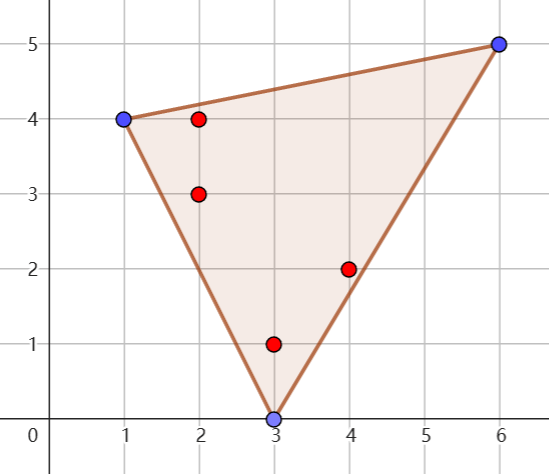
\includegraphics[width=.5\linewidth]{jpg.png}